\documentclass[aoas]{imsart}

\RequirePackage{amsthm,amsmath,amsfonts,amssymb}
\RequirePackage[authoryear]{natbib}
\RequirePackage{graphicx}
\RequirePackage{placeins}
\RequirePackage{enumitem}
\RequirePackage[colorlinks,citecolor=blue,urlcolor=blue,linkcolor=blue]{hyperref}

\startlocaldefs
\renewcommand{\P}{\mathbb{P}}
\newcommand{\E}{\mathbb{E}}
% Generated by scripts/manuscript/build-manuscript-artifacts.R; do not edit.
\providecommand{\ChicagoClock}{4:21}
\providecommand{\ChicagoDate}{November 5, 2019}
\providecommand{\ChicagoFinalAwayScore}{118}
\providecommand{\ChicagoFinalHomeScore}{112}
\providecommand{\ChicagoGameID}{401160742}
\providecommand{\ChicagoLoser}{Chicago Bulls}
\providecommand{\ChicagoMaxWP}{96.9\%}
\providecommand{\ChicagoMinutesRemaining}{16.4}
\providecommand{\ChicagoPIT}{0.968}
\providecommand{\ChicagoPeakAwayScore}{67}
\providecommand{\ChicagoPeakHomeScore}{85}
\providecommand{\ChicagoPeakLead}{18}
\providecommand{\ChicagoPeriod}{3}
\providecommand{\ChicagoSeason}{2020}
\providecommand{\ChicagoStartingWP}{71.2\%}
\providecommand{\ChicagoTailProbability}{3.2\%}
\providecommand{\ChicagoWinner}{Los Angeles Lakers}
\providecommand{\DyadicBootstrapReplicates}{9,999}
\providecommand{\DyadicBootstrapSeed}{20260815}
\providecommand{\NBACompletedGames}{8,290}
\providecommand{\NBACoverageRows}{
2018 & 1,230 & 1,230 & 1,222 & 8 \\
2019 & 1,230 & 1,230 & 1,230 & 0 \\
2020 & 1,062 & 1,059 & 1,053 & 6 \\
2021 & 1,112 & 1,080 & 1,080 & 0 \\
2022 & 1,241 & 1,230 & 1,230 & 0 \\
2023 & 1,231 & 1,230 & 1,230 & 0 \\
2024 & 1,233 & 1,231 & 1,231 & 0 \\
}
\providecommand{\NBACrossingNinetyCILower}{2.7\%}
\providecommand{\NBACrossingNinetyCIUpper}{4.7\%}
\providecommand{\NBACrossingNinetyEpisodes}{9,371}
\providecommand{\NBACrossingNinetyFiveAllCILower}{1.4\%}
\providecommand{\NBACrossingNinetyFiveAllCIUpper}{3.1\%}
\providecommand{\NBACrossingNinetyFiveAllEpisodes}{8,829}
\providecommand{\NBACrossingNinetyFiveAllGames}{8,266}
\providecommand{\NBACrossingNinetyFiveAllImplied}{4.1\%}
\providecommand{\NBACrossingNinetyFiveAllLoss}{6.4\%}
\providecommand{\NBACrossingNinetyFiveAllResidual}{2.3\%}
\providecommand{\NBACrossingNinetyFiveCILower}{1.4\%}
\providecommand{\NBACrossingNinetyFiveCIUpper}{3.2\%}
\providecommand{\NBACrossingNinetyFiveEpisodes}{8,663}
\providecommand{\NBACrossingNinetyFiveGames}{8,156}
\providecommand{\NBACrossingNinetyFiveImplied}{4.2\%}
\providecommand{\NBACrossingNinetyFiveLoss}{6.5\%}
\providecommand{\NBACrossingNinetyFiveResidual}{2.3\%}
\providecommand{\NBACrossingNinetyFiveStrictCILower}{1.5\%}
\providecommand{\NBACrossingNinetyFiveStrictCIUpper}{3.2\%}
\providecommand{\NBACrossingNinetyFiveStrictEpisodes}{8,654}
\providecommand{\NBACrossingNinetyFiveStrictGames}{8,154}
\providecommand{\NBACrossingNinetyFiveStrictImplied}{4.1\%}
\providecommand{\NBACrossingNinetyFiveStrictLoss}{6.4\%}
\providecommand{\NBACrossingNinetyFiveStrictResidual}{2.3\%}
\providecommand{\NBACrossingNinetyGames}{8,250}
\providecommand{\NBACrossingNinetyImplied}{8.8\%}
\providecommand{\NBACrossingNinetyLoss}{12.5\%}
\providecommand{\NBACrossingNinetyNineCILower}{0.1\%}
\providecommand{\NBACrossingNinetyNineCIUpper}{0.9\%}
\providecommand{\NBACrossingNinetyNineEpisodes}{7,660}
\providecommand{\NBACrossingNinetyNineGames}{7,598}
\providecommand{\NBACrossingNinetyNineImplied}{0.8\%}
\providecommand{\NBACrossingNinetyNineLoss}{1.3\%}
\providecommand{\NBACrossingNinetyNineResidual}{0.5\%}
\providecommand{\NBACrossingNinetyResidual}{3.7\%}
\providecommand{\NBADyadicCalendarGlobalD}{0.097}
\providecommand{\NBADyadicCalendarGlobalP}{\ensuremath{<0.001}}
\providecommand{\NBAEligibleGames}{8,290}
\providecommand{\NBAExcludePatchedGlobalD}{0.096}
\providecommand{\NBAExcludePatchedGlobalP}{\ensuremath{<0.001}}
\providecommand{\NBAExcludedExhibitionEvents}{10}
\providecommand{\NBAExcludedExhibitionFeeds}{5}
\providecommand{\NBAFixedClockExcluded}{11}
\providecommand{\NBAFixedClockGames}{8,265}
\providecommand{\NBAFixedClockLOCFCells}{195}
\providecommand{\NBAFixedClockLOCFRMS}{2.8\%}
\providecommand{\NBAFixedClockLOCFSignificantCells}{3}
\providecommand{\NBAFixedClockLinearCells}{196}
\providecommand{\NBAFixedClockLinearRMS}{2.7\%}
\providecommand{\NBAFixedClockLinearSignificantCells}{2}
\providecommand{\NBAFranchiseLinkedGlobalD}{0.097}
\providecommand{\NBAFranchiseLinkedGlobalP}{\ensuremath{<0.001}}
\providecommand{\NBAGames}{8,276}
\providecommand{\NBAGlobalCritical}{0.023}
\providecommand{\NBAGlobalD}{0.097}
\providecommand{\NBAGlobalDyadicP}{\ensuremath{<0.001}}
\providecommand{\NBALOSODMax}{0.102}
\providecommand{\NBALOSODMin}{0.093}
\providecommand{\NBALOSOTailMax}{1.5\%}
\providecommand{\NBALOSOTailMin}{1.2\%}
\providecommand{\NBALeaveSeasonRows}{
2018 & 7,054 & 0.093 & 1.5\% \\
2019 & 7,046 & 0.097 & 1.2\% \\
2020 & 7,223 & 0.094 & 1.3\% \\
2021 & 7,196 & 0.100 & 1.3\% \\
2022 & 7,046 & 0.102 & 1.3\% \\
2023 & 7,046 & 0.093 & 1.2\% \\
2024 & 7,045 & 0.101 & 1.5\% \\
}
\providecommand{\NBAMedianUpdatesPerGame}{466}
\providecommand{\NBAMinimumFeedCoverage}{99.3\%}
\providecommand{\NBAMissingCoverageRows}{
2018 & 1,222 & 8 & 99.3\% \\
2019 & 1,230 & 0 & 100.0\% \\
2020 & 1,053 & 6 & 99.4\% \\
2021 & 1,080 & 0 & 100.0\% \\
2022 & 1,230 & 0 & 100.0\% \\
2023 & 1,230 & 0 & 100.0\% \\
2024 & 1,231 & 0 & 100.0\% \\
}
\providecommand{\NBAMissingFeedGames}{14}
\providecommand{\NBANonfinalGames}{49}
\providecommand{\NBAPatchedGames}{16}
\providecommand{\NBAPublishedUpdates}{3,877,820}
\providecommand{\NBARawGlobalD}{0.097}
\providecommand{\NBARawGlobalP}{\ensuremath{<0.001}}
\providecommand{\NBARoundingLowerGlobalD}{0.095}
\providecommand{\NBARoundingLowerGlobalP}{\ensuremath{<0.001}}
\providecommand{\NBARoundingLowerTailNinetyFiveRate}{6.3\%}
\providecommand{\NBARoundingUpperGlobalD}{0.099}
\providecommand{\NBARoundingUpperGlobalP}{\ensuremath{<0.001}}
\providecommand{\NBARoundingUpperTailNinetyFiveRate}{6.6\%}
\providecommand{\NBAScheduledGames}{8,339}
\providecommand{\NBATailNinetyCILower}{1.4\%}
\providecommand{\NBATailNinetyCIUpper}{4.0\%}
\providecommand{\NBATailNinetyExcess}{2.7\%}
\providecommand{\NBATailNinetyFiveAtomRate}{0.00\%}
\providecommand{\NBATailNinetyFiveCILower}{0.4\%}
\providecommand{\NBATailNinetyFiveCIUpper}{2.3\%}
\providecommand{\NBATailNinetyFiveExcess}{1.3\%}
\providecommand{\NBATailNinetyFiveRate}{6.3\%}
\providecommand{\NBATailNinetyFiveStrictRate}{6.3\%}
\providecommand{\NBATailNinetyNineCILower}{-0.3\%}
\providecommand{\NBATailNinetyNineCIUpper}{0.5\%}
\providecommand{\NBATailNinetyNineExcess}{0.1\%}
\providecommand{\NBATailNinetyNineRate}{1.1\%}
\providecommand{\NBATailNinetyRate}{12.7\%}
\providecommand{\NBATiedGames}{0}
\providecommand{\NBAUpdateQOne}{447}
\providecommand{\NBAUpdateQThree}{488}
\providecommand{\NFLCompletedGames}{1,855}
\providecommand{\NFLCoverageRows}{
2018 & 256 & 254 & 254 & 0 \\
2019 & 256 & 255 & 255 & 0 \\
2020 & 256 & 255 & 255 & 0 \\
2021 & 272 & 271 & 271 & 0 \\
2022 & 272 & 269 & 269 & 0 \\
2023 & 272 & 272 & 272 & 0 \\
2024 & 272 & 272 & 272 & 0 \\
}
\providecommand{\NFLCrossingNinetyCILower}{-0.9\%}
\providecommand{\NFLCrossingNinetyCIUpper}{2.8\%}
\providecommand{\NFLCrossingNinetyEpisodes}{1,974}
\providecommand{\NFLCrossingNinetyFiveAllCILower}{-0.2\%}
\providecommand{\NFLCrossingNinetyFiveAllCIUpper}{2.7\%}
\providecommand{\NFLCrossingNinetyFiveAllEpisodes}{1,932}
\providecommand{\NFLCrossingNinetyFiveAllGames}{1,847}
\providecommand{\NFLCrossingNinetyFiveAllImplied}{3.2\%}
\providecommand{\NFLCrossingNinetyFiveAllLoss}{4.4\%}
\providecommand{\NFLCrossingNinetyFiveAllResidual}{1.2\%}
\providecommand{\NFLCrossingNinetyFiveCILower}{-0.2\%}
\providecommand{\NFLCrossingNinetyFiveCIUpper}{2.9\%}
\providecommand{\NFLCrossingNinetyFiveEpisodes}{1,842}
\providecommand{\NFLCrossingNinetyFiveGames}{1,772}
\providecommand{\NFLCrossingNinetyFiveImplied}{3.3\%}
\providecommand{\NFLCrossingNinetyFiveLoss}{4.6\%}
\providecommand{\NFLCrossingNinetyFiveResidual}{1.3\%}
\providecommand{\NFLCrossingNinetyFiveStrictCILower}{-0.2\%}
\providecommand{\NFLCrossingNinetyFiveStrictCIUpper}{2.9\%}
\providecommand{\NFLCrossingNinetyFiveStrictEpisodes}{1,841}
\providecommand{\NFLCrossingNinetyFiveStrictGames}{1,771}
\providecommand{\NFLCrossingNinetyFiveStrictImplied}{3.3\%}
\providecommand{\NFLCrossingNinetyFiveStrictLoss}{4.6\%}
\providecommand{\NFLCrossingNinetyFiveStrictResidual}{1.3\%}
\providecommand{\NFLCrossingNinetyGames}{1,818}
\providecommand{\NFLCrossingNinetyImplied}{7.6\%}
\providecommand{\NFLCrossingNinetyLoss}{8.5\%}
\providecommand{\NFLCrossingNinetyNineCILower}{0.2\%}
\providecommand{\NFLCrossingNinetyNineCIUpper}{2.2\%}
\providecommand{\NFLCrossingNinetyNineEpisodes}{1,705}
\providecommand{\NFLCrossingNinetyNineGames}{1,686}
\providecommand{\NFLCrossingNinetyNineImplied}{0.5\%}
\providecommand{\NFLCrossingNinetyNineLoss}{1.6\%}
\providecommand{\NFLCrossingNinetyNineResidual}{1.1\%}
\providecommand{\NFLCrossingNinetyResidual}{0.9\%}
\providecommand{\NFLDyadicCalendarGlobalD}{0.015}
\providecommand{\NFLDyadicCalendarGlobalP}{\ensuremath{0.856}}
\providecommand{\NFLEligibleGames}{1,848}
\providecommand{\NFLExcludePatchedGlobalD}{0.014}
\providecommand{\NFLExcludePatchedGlobalP}{\ensuremath{0.769}}
\providecommand{\NFLFixedClockExcluded}{0}
\providecommand{\NFLFixedClockGames}{1,848}
\providecommand{\NFLFixedClockLOCFCells}{197}
\providecommand{\NFLFixedClockLOCFRMS}{2.6\%}
\providecommand{\NFLFixedClockLOCFSignificantCells}{8}
\providecommand{\NFLFixedClockLinearCells}{197}
\providecommand{\NFLFixedClockLinearRMS}{2.9\%}
\providecommand{\NFLFixedClockLinearSignificantCells}{8}
\providecommand{\NFLFranchiseLinkedGlobalD}{0.015}
\providecommand{\NFLFranchiseLinkedGlobalP}{\ensuremath{0.705}}
\providecommand{\NFLGames}{1,848}
\providecommand{\NFLGlobalCritical}{0.047}
\providecommand{\NFLGlobalD}{0.015}
\providecommand{\NFLGlobalDyadicP}{\ensuremath{0.736}}
\providecommand{\NFLLOSODMax}{0.025}
\providecommand{\NFLLOSODMin}{0.008}
\providecommand{\NFLLOSOTailMax}{0.0\%}
\providecommand{\NFLLOSOTailMin}{-1.0\%}
\providecommand{\NFLLeaveSeasonRows}{
2018 & 1,594 & 0.017 & -0.7\% \\
2019 & 1,593 & 0.013 & -0.3\% \\
2020 & 1,593 & 0.014 & -1.0\% \\
2021 & 1,577 & 0.013 & -0.3\% \\
2022 & 1,579 & 0.008 & -0.8\% \\
2023 & 1,576 & 0.024 & -0.4\% \\
2024 & 1,576 & 0.025 & 0.0\% \\
}
\providecommand{\NFLMedianUpdatesPerGame}{175}
\providecommand{\NFLMinimumFeedCoverage}{100.0\%}
\providecommand{\NFLMissingCoverageRows}{
2018 & 254 & 0 & 100.0\% \\
2019 & 255 & 0 & 100.0\% \\
2020 & 255 & 0 & 100.0\% \\
2021 & 271 & 0 & 100.0\% \\
2022 & 269 & 0 & 100.0\% \\
2023 & 272 & 0 & 100.0\% \\
2024 & 272 & 0 & 100.0\% \\
}
\providecommand{\NFLMissingFeedGames}{0}
\providecommand{\NFLNonfinalGames}{1}
\providecommand{\NFLPatchedGames}{4}
\providecommand{\NFLPublishedUpdates}{325,922}
\providecommand{\NFLRawGlobalD}{0.015}
\providecommand{\NFLRawGlobalP}{\ensuremath{0.735}}
\providecommand{\NFLRoundingLowerGlobalD}{0.013}
\providecommand{\NFLRoundingLowerGlobalP}{\ensuremath{0.775}}
\providecommand{\NFLRoundingLowerTailNinetyFiveRate}{4.5\%}
\providecommand{\NFLRoundingUpperGlobalD}{0.016}
\providecommand{\NFLRoundingUpperGlobalP}{\ensuremath{0.679}}
\providecommand{\NFLRoundingUpperTailNinetyFiveRate}{4.5\%}
\providecommand{\NFLScheduledGames}{1,856}
\providecommand{\NFLTailNinetyCILower}{-3.5\%}
\providecommand{\NFLTailNinetyCIUpper}{0.7\%}
\providecommand{\NFLTailNinetyExcess}{-1.5\%}
\providecommand{\NFLTailNinetyFiveAtomRate}{0.00\%}
\providecommand{\NFLTailNinetyFiveCILower}{-2.0\%}
\providecommand{\NFLTailNinetyFiveCIUpper}{1.1\%}
\providecommand{\NFLTailNinetyFiveExcess}{-0.5\%}
\providecommand{\NFLTailNinetyFiveRate}{4.5\%}
\providecommand{\NFLTailNinetyFiveStrictRate}{4.5\%}
\providecommand{\NFLTailNinetyNineCILower}{-0.3\%}
\providecommand{\NFLTailNinetyNineCIUpper}{1.5\%}
\providecommand{\NFLTailNinetyNineExcess}{0.5\%}
\providecommand{\NFLTailNinetyNineRate}{1.5\%}
\providecommand{\NFLTailNinetyRate}{8.5\%}
\providecommand{\NFLTiedGames}{7}
\providecommand{\NFLUpdateQOne}{167}
\providecommand{\NFLUpdateQThree}{185}
\providecommand{\SimulationBaseGrid}{1,000}
\providecommand{\SimulationCoarseningN}{50,000}
\providecommand{\ValidationInnerReplicates}{399}
\providecommand{\ValidationNBARhoFiftyDyadic}{4.4\%}
\providecommand{\ValidationNBARhoTwentyFiveDyadic}{3.2\%}
\providecommand{\ValidationNBARhoZeroDyadic}{0.0\%}
\providecommand{\ValidationNFLRhoFiftyDyadic}{3.2\%}
\providecommand{\ValidationNFLRhoTwentyFiveDyadic}{0.8\%}
\providecommand{\ValidationNFLRhoZeroDyadic}{0.0\%}
\providecommand{\ValidationOuterSamples}{250}
\theoremstyle{plain}
\newtheorem{theorem}{Theorem}[section]
\newtheorem{proposition}[theorem]{Proposition}
\newtheorem{corollary}[theorem]{Corollary}
\renewcommand{\thesection}{S\arabic{section}}
\renewcommand{\thesubsection}{S\arabic{section}.\arabic{subsection}}
\counterwithin{table}{section}
\counterwithin{figure}{section}
\renewcommand{\thetable}{\thesection.\arabic{table}}
\renewcommand{\thefigure}{\thesection.\arabic{figure}}
\endlocaldefs

\begin{document}
\begin{frontmatter}
\title{Supplementary Material for The Blown Lead Paradox: A Pathwise Calibration Benchmark for Win Probability Forecasts}
\runtitle{Supplementary Material for The Blown Lead Paradox}

\begin{aug}
\author[A]{\fnms{Jonathan}~\snm{Pipping-Gam\'on}\ead[label=e1]{jpipping@wharton.upenn.edu}\orcid{0009-0000-2540-2469}}
\and
\author[A]{\fnms{Abraham J.}~\snm{Wyner}\ead[label=e2]{ajw@wharton.upenn.edu}}
\address[A]{Department of Statistics, University of Pennsylvania \printead[presep={,\ }]{e1,e2}}
\end{aug}
\end{frontmatter}

\setcounter{section}{0}
\section{Proofs of Discrete-Time Results} \label{app:discrete-proofs}

Throughout, $(p_k)_{k=0}^N$ is a bounded martingale with $p_0\in(0,1)$ and terminal value $p_N=Y\in\{0,1\}$.
For $x\in(0,1]$, define the first-passage time
\[
\tau_x := \inf\{k\in\{0,1,\dots,N\}: p_k\ge x\},
\]
with $\inf\varnothing := N+1$.

\subsection{Unconditional distribution of \texorpdfstring{$M_N$}{M N}}

\begin{theorem}[Discrete-time unconditional bound] \label{thm:supp-discrete-unconditional}
Let $M_N=\max_{0\le k\le N} p_k$. For $x\in[p_0,1)$,
\[
\P(M_N<x)\;\ge\;1-\frac{p_0}{x},
\]
and hence $F_{M_N}(x)=\P(M_N\le x)\ge 1-p_0/x$.
The strict-threshold bound is an equality if $p_{\tau_x}=x$ a.s.\ on $\{\tau_x\le N\}$; equality for $F_{M_N}(x)$ additionally requires $\P(M_N=x)=0$.
For $x<p_0$, $F_{M_N}(x)=0$.
Moreover, $M_N$ has an atom at $1$ with $\P(M_N=1)=p_0$.
\end{theorem}

\begin{proof}
If $x<p_0$ then $M_N\ge p_0>x$ a.s., hence $F_{M_N}(x)=0$.

Fix $x\in[p_0,1)$. By optional stopping for the bounded martingale $(p_k)$ at $\tau_x\wedge N$,
\[
\E[p_{\tau_x\wedge N}] = p_0.
\]
Decompose $p_{\tau_x\wedge N}=p_{\tau_x}\mathbf 1\{\tau_x\le N\}+p_N\mathbf 1\{\tau_x>N\}$.
On $\{\tau_x\le N\}$ we have $p_{\tau_x}\ge x$.
Therefore,
\[
p_0
= \E[p_{\tau_x}\mathbf 1\{\tau_x\le N\}] + \E[p_N\mathbf 1\{\tau_x>N\}]
\;\ge\; x\,\P(\tau_x\le N).
\]
Since $\{\tau_x\le N\}=\{M_N\ge x\}$, this yields
\[
\P(M_N\ge x)\le \frac{p_0}{x}\qquad\Rightarrow\qquad
\P(M_N<x)\ge 1-\frac{p_0}{x}.
\]
Equality in the strict-threshold bound holds when $p_{\tau_x}=x$ a.s.\ on $\{\tau_x\le N\}$.
Because $F_{M_N}(x)=\P(M_N<x)+\P(M_N=x)$, the corresponding CDF equality also requires no atom at $x$.

Finally, $M_N=1$ iff $p_N=1$ iff $Y=1$, so $\P(M_N=1)=p_0$.
\end{proof}

\subsection{Conditional distribution of \texorpdfstring{$M_N$ given $Y=0$}{M N given Y=0}}

\begin{theorem}[Discrete-time conditional bound] \label{thm:supp-discrete-conditional}
For $x\in[p_0,1)$,
\[
\P(M_N<x\mid Y=0)
\;\ge\;
1-\Big(\frac{p_0}{1-p_0}\Big)\Big(\frac{1-x}{x}\Big),
\]
and hence the same bound holds for $F_{M_N\mid Y=0}(x)=\P(M_N\le x\mid Y=0)$.
The strict-threshold bound is an equality under the same no-overshoot condition as in Theorem~\ref{thm:supp-discrete-unconditional}; CDF equality additionally requires $\P(M_N=x\mid Y=0)=0$.
For $x<p_0$, $F_{M_N\mid Y=0}(x)=0$.
\end{theorem}

\begin{proof}
Fix $x\in[p_0,1)$. Decompose $\P(M_N\ge x)$ by $Y$:
\[
\P(M_N\ge x)=\P(M_N\ge x, Y=1)+\P(M_N\ge x, Y=0).
\]
On $\{Y=1\}$ we have $p_N=1\ge x$, hence $\{Y=1\}\subseteq\{M_N\ge x\}$ and
\begin{align*}
\P(M_N\ge x)
&=\P(Y=1)+\P(Y=0)\P(M_N\ge x\mid Y=0) \\
&=p_0+(1-p_0)\P(M_N\ge x\mid Y=0).
\end{align*}
By Theorem~\ref{thm:supp-discrete-unconditional}, $\P(M_N\ge x)\le p_0/x$, so
\[
\frac{p_0}{x}\;\ge\; p_0 + (1-p_0)\P(M_N\ge x\mid Y=0),
\]
which rearranges to
\[
\P(M_N\ge x\mid Y=0)\;\le\;\Big(\frac{p_0}{1-p_0}\Big)\Big(\frac{1-x}{x}\Big).
\]
Taking complements gives the stated strict-threshold bound; the ordinary CDF bound follows because $\P(M_N\le x\mid Y=0)\ge\P(M_N<x\mid Y=0)$.
\end{proof}

\begin{proposition}[Discrete-time correction identity]
For $x\in(p_0,1)$,
\begin{align*}
\P(M_N\ge x\mid Y=0)
={}&\frac{p_0}{1-p_0}\cdot\frac{1-x}{x} \\
&-\frac{1}{x(1-p_0)}
  \E\!\big[(p_{\tau_x}-x)\mathbf 1\{\tau_x<N\}\big] \\
&-\frac{1-x}{x(1-p_0)}\,\P(\tau_x=N).
\end{align*}
\end{proposition}

\begin{proof}
Fix $x\in(p_0,1)$. Since $x<1$, the event $\{Y=1\}$ is contained in $\{\tau_x\le N\}$, so
\[
\P(\tau_x\le N)=\P(Y=1)+(1-p_0)\P(M_N\ge x\mid Y=0).
\]
Optional stopping at $\tau_x\wedge N$ gives
\[
p_0=\E[p_{\tau_x\wedge N}]
=\E[p_{\tau_x}\mathbf 1\{\tau_x\le N\}]
=x\,\P(\tau_x\le N)+\E\!\big[(p_{\tau_x}-x)\mathbf 1\{\tau_x\le N\}\big].
\]
Combining the two displays and rearranging yields
\[
\P(M_N\ge x\mid Y=0)
=\frac{p_0}{1-p_0}\cdot\frac{1-x}{x}
-\frac{1}{x(1-p_0)}\,\E\!\big[(p_{\tau_x}-x)\mathbf 1\{\tau_x\le N\}\big].
\]
Finally,
\[
\E\!\big[(p_{\tau_x}-x)\mathbf 1\{\tau_x\le N\}\big]
=\E\!\big[(p_{\tau_x}-x)\mathbf 1\{\tau_x< N\}\big]+(1-x)\P(\tau_x=N),
\]
because $\tau_x=N$ implies $p_{\tau_x}=p_N=1$.
Substituting gives the stated decomposition.
\end{proof}

\section{Proofs of Continuous-Path Results} \label{app:continuous-proofs}

Let $(p_t)_{t\in[0,1]}$ be a bounded martingale with $p_0\in(0,1)$ and $p_1=Y\in\{0,1\}$, and assume path continuity.
Define $M=\sup_{t\in[0,1]}p_t$ and $\tau_x=\inf\{t\in[0,1]: p_t\ge x\}$.

\subsection{Unconditional distribution of \texorpdfstring{$M$}{M}}

\begin{theorem}[Continuous-path unconditional] \label{thm:supp-continuous-unconditional}
For $x\in[p_0,1)$,
\[
F_M(x)=\P(M\le x)=1-\frac{p_0}{x},
\]
and $F_M(x)=0$ for $x<p_0$, while $F_M(1)=1$.
In particular, $\P(M=1)=p_0$.
\end{theorem}

\begin{proof}
If $x<p_0$ then $M\ge p_0>x$ a.s.

Fix $x\in[p_0,1)$. Optional stopping at $\tau_x\wedge 1$ yields $\E[p_{\tau_x\wedge 1}]=p_0$.
By continuity, on $\{\tau_x<1\}$ we have $p_{\tau_x}=x$, and on $\{\tau_x\ge 1\}$ we have $p_1=Y$.
Thus
\[
p_0 = x\,\P(\tau_x<1) + \E[Y\mathbf 1\{\tau_x\ge 1\}].
\]
But if $Y=1$, continuity and $p_1=1>x$ imply that $p_t\ge x$ for some $t<1$, and hence $\tau_x<1$; therefore
$\E[Y\mathbf 1\{\tau_x\ge 1\}]=0$ for $x<1$.
Therefore $p_0 = x\,\P(\tau_x<1)$, i.e.\ $\P(M\ge x)=\P(\tau_x<1)=p_0/x$.
Because this tail is continuous in $x$ on $[p_0,1)$, $M$ has no atoms there.
Thus $\P(M\le x)=\P(M<x)=1-p_0/x$ on that interval.
Finally, $M=1$ iff $Y=1$, so $\P(M=1)=p_0$.
\end{proof}

\subsection{Conditional distribution of \texorpdfstring{$M$ given $Y=0$}{M given Y=0}}

\begin{theorem}[Continuous-path conditional] \label{thm:supp-continuous-conditional}
For $x\in[p_0,1)$,
\[
F_{M\mid Y=0}(x)=\P(M\le x\mid Y=0)
=
1-\Big(\frac{p_0}{1-p_0}\Big)\Big(\frac{1-x}{x}\Big),
\]
and $F_{M\mid Y=0}(x)=0$ for $x<p_0$, while $F_{M\mid Y=0}(1)=1$.
\end{theorem}

\begin{proof}
Fix $x\in[p_0,1)$. As before,
\[
\P(M\ge x)=\P(Y=1)+(1-p_0)\P(M\ge x\mid Y=0)=p_0+(1-p_0)\P(M\ge x\mid Y=0).
\]
By Theorem~\ref{thm:supp-continuous-unconditional}, $\P(M\ge x)=p_0/x$, hence
\[
\frac{p_0}{x}=p_0+(1-p_0)\P(M\ge x\mid Y=0)
\quad\Rightarrow\quad
\P(M\ge x\mid Y=0)=\Big(\frac{p_0}{1-p_0}\Big)\Big(\frac{1-x}{x}\Big).
\]
This conditional tail is continuous in $x$ below one, so it has no atoms there; taking complements yields the stated CDF.
Finally, on $\{Y=0\}$ the process cannot attain $1$ (if $p_t=1$ then $\P(Y=1\mid\mathcal F_t)=1$), so $M<1$ a.s.\ and $F_{M\mid Y=0}(1)=1$.
\end{proof}

\section{Distribution of \texorpdfstring{$M_\lambda$}{M\_lambda} (Two Teams)} \label{app:two-player-derivation}

Let $(p_t)$ and $(q_t)$ be the two teams' win-probability martingales, where $q_t = 1 - p_t$ and $p_0 = \P(Y=1)$; assume $p_0 \ge 0.5$ without loss of generality.
The maximum win probability attained by the eventual loser is
\begin{equation} \label{eq:supp-M-lambda-def}
    M_\lambda \equiv \sup_{0 \leq t \leq 1} \Big( p_t \boldsymbol{1}\{Y = 0\} + q_t \boldsymbol{1}\{Y = 1\} \Big).
\end{equation}
By the law of total probability,
\begin{align} \label{eq:supp-M-lambda-total-prob}
    F_{M_\lambda}(x) = \P(M_\lambda \le x) &= \P(M_\lambda \le x \mid Y=0) (1-p_0) + \P(M_\lambda \le x \mid Y=1) p_0.
\end{align}

When team~A loses, Theorem~\ref{thm:supp-continuous-conditional} gives
\begin{align}
    F_{M_\lambda \mid Y=0}(x) = \P(M_\lambda \le x \mid Y = 0) &=
    \begin{cases}
        0 & \text{for } x < p_0, \\
        1 - \left(\frac{p_0}{1-p_0}\right) \left(\frac{1-x}{x}\right) & \text{for } x \in [p_0,1), \\
        1 & \text{for } x = 1.
    \end{cases} \label{eq:supp-M-lambda-A}
\end{align}
Applying the same formula with $p_0$ replaced by $1-p_0$ gives
\begin{align}
    F_{M_\lambda \mid Y=1}(x) = \P(M_\lambda \le x \mid Y = 1) &=
    \begin{cases}
        0 & \text{for } x < 1-p_0, \\
        1 - \left(\frac{1-p_0}{p_0}\right) \left(\frac{1-x}{x}\right) & \text{for } x \in [1-p_0,1), \\
        1 & \text{for } x = 1.
    \end{cases} \label{eq:supp-M-lambda-B}
\end{align}

With $p_0 \ge 0.5$ (team~A favored), substituting \eqref{eq:supp-M-lambda-A} and \eqref{eq:supp-M-lambda-B} into \eqref{eq:supp-M-lambda-total-prob} gives three regions:
\begin{enumerate}[leftmargin=*]
    \item For $0 \le x < 1-p_0$, neither \eqref{eq:supp-M-lambda-A} nor \eqref{eq:supp-M-lambda-B} contributes, so $F_{M_\lambda}(x) = 0$.

    \item For $1-p_0 \le x < p_0$, only \eqref{eq:supp-M-lambda-B} contributes:
    \begin{align*}
        F_{M_\lambda}(x) &= (1-p_0) \cdot 0 + p_0 \cdot \left[1 - \left(\frac{1-p_0}{p_0}\right) \left(\frac{1-x}{x}\right)\right] \\
        &= p_0 - (1-p_0)\left(\frac{1-x}{x}\right) = 1 - \frac{1-p_0}{x}.
    \end{align*}

    \item For $x \ge p_0$, both \eqref{eq:supp-M-lambda-A} and \eqref{eq:supp-M-lambda-B} contribute:
    \begin{align*}
        F_{M_\lambda}(x) &= (1-p_0)\left[1 - \left(\frac{p_0}{1-p_0}\right) \left(\frac{1-x}{x}\right)\right] + p_0\left[1 - \left(\frac{1-p_0}{p_0}\right) \left(\frac{1-x}{x}\right)\right] \\
        &= \left[(1-p_0) - p_0\left(\frac{1-x}{x}\right)\right] + \left[p_0 - (1-p_0)\left(\frac{1-x}{x}\right)\right] \\
        &= 1 - \frac{1-x}{x} = \frac{2x-1}{x} = 2 - \frac{1}{x}.
    \end{align*}
\end{enumerate}

Combining the three regions gives the piecewise cumulative distribution function
\begin{equation*}
    F_{M_\lambda}(x) = \P(M_\lambda \le x) = \begin{cases}
        0 & \text{for } 0 \le x < 1-p_0, \\[0.5em]
        1 - \frac{1-p_0}{x} & \text{for } 1-p_0 \le x < p_0, \\[0.5em]
        2 - \frac{1}{x} & \text{for } p_0 \le x < 1, \\[0.5em]
        1 & \text{for } x = 1.
    \end{cases}
\end{equation*}

\section{Numerical Benchmarks} \label{sec:supp-benchmarks}

The piecewise CDF in Supplementary Section~\ref{app:two-player-derivation} gives the selected values in Table~\ref{tab:supp-numerical-benchmarks}.
When the peak threshold satisfies $x\ge p_0$, the tail is universal:
\[
\P(M_\lambda\ge x)=\frac{1}{x}-1.
\]
In the intermediate region, $1-p_0\le x<p_0$, the corresponding probability is $(1-p_0)/x$.
The first three rows follow a game with $p_0=2/3$ across the boundary between these regions; the remaining rows give the practically important upper-tail thresholds.
For discretely reported paths, these continuous-path probabilities are conservative upper bounds.

\begin{table}[!tbp]
\centering
\small
\caption{Selected benchmark probabilities for the eventual loser's peak.}
\label{tab:supp-numerical-benchmarks}
\begin{tabular}{lccc}
\hline
Case & Starting favorite & Peak threshold $x$ & $\P(M_\lambda\ge x)$ \\
\hline
Intermediate region & $p_0=2/3$ & $1/2$ & $2/3$ \\
Universal boundary & $p_0=2/3$ & $2/3$ & $1/2$ \\
Universal tail & $p_0=2/3$ & $3/4$ & $1/3$ \\
Universal tail & $p_0\le 0.90$ & $0.90$ & $1/9\;(0.111)$ \\
Universal tail & $p_0\le 0.95$ & $0.95$ & $1/19\;(0.0526)$ \\
Universal tail & $p_0\le 0.99$ & $0.99$ & $1/99\;(0.0101)$ \\
\hline
\end{tabular}
\end{table}

\section{Dependence Validity and Bootstrap} \label{sec:supp-inference}

Intervals and $p$-values in Sections~\ref{sec:supp-inference}--\ref{sec:supp-results} use $B=\DyadicBootstrapReplicates$ season-stratified dyadic draws with seed \DyadicBootstrapSeed.

\subsection{Exchangeable-array specialization}

The empirical-process bootstrap theorem of \citet{DaveziesDHAultfoeuilleGuyonvarch2021} and its multiple-observations-per-dyad extension cover zero or repeated sports matches between a pair.
The following corollary specializes those results to an equal-game empirical CDF with within-season normalization.

For season $s$, let $n_s$ be the number of teams, $N_{s,ab}$ the number of games between teams $a<b$, and $U_{s,ab\ell}$ the benchmark score in meeting $\ell$.
For $h_t(u)=\mathbf 1\{u<t\}$, define the empirical numerator and denominator
\[
\widehat A_s(t)
=\binom{n_s}{2}^{-1}
  \sum_{a<b}\sum_{\ell=1}^{N_{s,ab}}h_t(U_{s,ab\ell}),
\qquad
\widehat B_s
=\binom{n_s}{2}^{-1}\sum_{a<b}N_{s,ab}.
\]
The strict empirical CDF among games in season $s$ is therefore
\[
\widehat F_s(t-)=\frac{\widehat A_s(t)}{\widehat B_s}.
\]
Its population counterpart is $F_s(t-)=A_s(t)/B_s$, where
\[
A_s(t)=\E\!\left[\sum_{\ell=1}^{N_{s,12}}h_t(U_{s,12\ell})\right],
\qquad
B_s=\E[N_{s,12}].
\]
Let $\omega_{s,n}\ge0$ be fixed stratification weights, with $\sum_s\omega_{s,n}=1$ and $\omega_{s,n}\to\omega_s$.
The application conditions on the observed season composition and sets these weights to each season's share of analyzed games.
Thus
\[
\widehat F(t-)=\sum_{s=1}^S\omega_{s,n}\widehat F_s(t-),
\qquad
F_{\omega,n}(t-)=\sum_{s=1}^S\omega_{s,n}F_s(t-).
\]

Within season $s$, let $(W_{s1},\ldots,W_{sn_s})$ be multinomial team multiplicities from $n_s$ draws.
The bootstrap analogues are
\begin{align*}
\widehat A_s^*(t)
&=\binom{n_s}{2}^{-1}
  \sum_{a<b}W_{sa}W_{sb}
  \sum_{\ell=1}^{N_{s,ab}}h_t(U_{s,ab\ell}),\\
\widehat B_s^*
&=\binom{n_s}{2}^{-1}
  \sum_{a<b}W_{sa}W_{sb}N_{s,ab},
\qquad
\widehat F_s^*(t-)=\frac{\widehat A_s^*(t)}{\widehat B_s^*},
\end{align*}
and $\widehat F^*(t-)=\sum_s\omega_{s,n}\widehat F_s^*(t-)$.
This ratio is exactly the CDF obtained by normalizing the raw game weights $W_{sa}W_{sb}$ within season.

\begin{corollary}[CDF specialization of the exchangeable-array bootstrap] \label{cor:dyadic-cdf}
Let the number of seasons $S$ be fixed, $n_{\min}=\min_s n_s\to\infty$, and $n_{\min}/n_s\to\kappa_s\in(0,1]$.
Within each season, suppose
\[
\bigl(N_{s,ab},(U_{s,ab\ell})_{\ell\ge1}\bigr)_{a<b}
\]
is jointly exchangeable and dissociated under team relabeling, and suppose the season arrays are independent.
Assume $N_{s,ab}\le C<\infty$ almost surely and $B_s>0$.
Assume also that the first-order dyadic projection of the normalized CDF process is nondegenerate, meaning that its limiting covariance function is not identically zero.
Then, in $\ell^\infty([0,1])$,
\[
\sqrt{n_{\min}}\{\widehat F(t-)-F_{\omega,n}(t-)\}
\rightsquigarrow \mathbb G(t),
\]
and, conditionally on the observed arrays,
\[
\sqrt{n_{\min}}\{\widehat F^*(t-)-\widehat F(t-)\}
\rightsquigarrow \mathbb G(t).
\]
Consequently, at continuity points of the limiting supremum law, the conditional distribution of
\[
\sqrt{n_{\min}}\sup_t\{\widehat F(t-)-\widehat F^*(t-)\}
\]
consistently estimates the distribution of
\[
\sqrt{n_{\min}}\sup_t\{F_{\omega,n}(t-)-\widehat F(t-)\}.
\]
\end{corollary}

\begin{proof}
The class
\[
\mathcal H_+=\{u\mapsto\mathbf 1(u<t):t\in[0,1]\}\cup\{1\}
\]
is a pointwise measurable VC class with bounded envelope: rational thresholds form a countable pointwise-dense subclass.
Parts 2 and 3 of Supplemental Theorem S1 in \citet{DaveziesDHAultfoeuilleGuyonvarch2021} therefore give joint weak convergence of
$\sqrt{n_s}(\widehat A_s-A_s,\widehat B_s-B_s)$ and its multinomial-team bootstrap counterpart.
The bounded cell count supplies the extension's moment conditions.
An unordered symmetric dyad can be embedded in the theorem's ordered-array notation by assigning the same cell to $(a,b)$ and $(b,a)$; the common factor of two cancels from the CDF ratio.

Because $B_s>0$, the map $\Psi(A,B)=A/B$ is Hadamard differentiable, with derivative
\[
\dot\Psi_{(A_s,B_s)}(\alpha,\beta)
=\frac{\alpha}{B_s}-\frac{A_s\beta}{B_s^2}.
\]
The bootstrap functional delta method therefore gives the two process limits for each normalized season CDF.
The second term carries the denominator fluctuation into the normalized process.
A finite independent weighted sum, together with $n_{\min}/n_s\to\kappa_s$, gives the pooled limits.
Finally, $f\mapsto\sup_t\{-f(t)\}$ is Lipschitz on $\ell^\infty([0,1])$, which gives the last assertion directly, without a symmetry argument.
\end{proof}

\begin{corollary}[Conservative upper-tail test] \label{cor:conservative-test}
Suppose in addition that the discrete-feed null satisfies $F_{\omega,n}(t-)\ge t$ for every $t\in[0,1]$.
Let $c_{1-\alpha}^*$ be the conditional $(1-\alpha)$ quantile of the scaled recentered bootstrap statistic in Corollary~\ref{cor:dyadic-cdf}.
Define
\[
D_n^{\mathrm{upper}}=\sup_t\{t-\widehat F(t-)\}
\]
and reject when $\sqrt{n_{\min}}D_n^{\mathrm{upper}}>c_{1-\alpha}^*$.
This test has asymptotic size at most $\alpha$ whenever the limiting supremum distribution is continuous at its $(1-\alpha)$ quantile.
\end{corollary}

\begin{proof}
Under the null,
\[
t-\widehat F(t-)
\le F_{\omega,n}(t-)-\widehat F(t-)
\]
pointwise.
The result follows by taking suprema and applying Corollary~\ref{cor:dyadic-cdf}.
\end{proof}

Corollaries~\ref{cor:dyadic-cdf}--\ref{cor:conservative-test} use a dense-array asymptotic and a nondegenerate first-order dyadic projection.
A vanishing projection can produce a second-order limit and conservative pigeonhole resampling; more generally, \citet{Menzel2021} rules out uniform bootstrap consistency across all multiway-dependence regimes.
Professional schedules have fixed conference and division structures, and franchises persist across seasons.
Section~\ref{sec:supp-validation} evaluates finite-sample size on the observed schedules, and the franchise-linked specification in Table~\ref{tab:supp-specification} carries team effects across seasons.

\subsection{Season-stratified dyadic pigeonhole bootstrap}

Write game $g$ in season $s$ as the dyad $(a_g,b_g)$.
The resampling algorithm is:
\begin{enumerate}[leftmargin=2em]
\item Within each season, sample its observed teams multinomially with replacement and record team multiplicities $W_{sa}$.
\item Give game $g$ raw weight $W_{s a_g}W_{s b_g}$. Repeat meetings between the same teams therefore receive the same endpoint weight. If a season draw assigns zero total weight to its observed schedule, redraw that season.
\item Normalize the positive game weights within season to sum to that season's observed number of contributions. This retains the empirical season composition while allowing arbitrary dependence among games that share a team.
\item Reuse the same team multiplicities for the PIT process, tail rates, first-crossing residuals, and fixed-clock calibration cells.
\end{enumerate}
This applies Owen's pigeonhole principle---resampling indexing units rather than treating cells as independent---to a symmetric dyadic schedule \citep{Owen2007}.
The exchangeable-array empirical-process results of \citet{DaveziesDHAultfoeuilleGuyonvarch2021} cover recentered empirical CDF and Kolmogorov--Smirnov processes for dyads, including repeated observations between the same pair.

For tied PIT scores $u_1,\ldots,u_n$, the observed upper statistic is computed exactly as
\[
D_n^{\mathrm{upper}}
=\max_{u\in\{u_1,\ldots,u_n\}}\{u-\hat F_U(u-)\}.
\]
For bootstrap draw $b$, let $\hat F_{U,b}^*$ be the season-normalized weighted CDF and calculate
\[
D_{n,b}^*=\sup_t\{\hat F_U(t)-\hat F_{U,b}^*(t)\}.
\]
For the common observed support, this right-continuous supremum equals the strict-CDF supremum in Corollary~\ref{cor:dyadic-cdf}: both empirical CDFs have the same total mass, so their right-limit and left-limit differences run through the same values, with zero at opposite endpoints.
The finite-bootstrap $p$-value is $(1+\sum_b\mathbf 1\{D_{n,b}^*\ge D_n^{\mathrm{upper}}\})/(B+1)$.

\section{Published Feeds and Fixed-Time Calibration} \label{sec:supp-data}

Both applications contain completed regular-season games only.
NFL seasons are labeled by starting year and include January games from the following calendar year; NBA seasons are labeled by ending year.
Because ESPN's NBA season-type field also includes All-Star exhibitions, both participants must be NBA franchises; this excludes \NBAExcludedExhibitionEvents{} All-Star or Rising Stars events, including \NBAExcludedExhibitionFeeds{} with usable probability paths.
Table~\ref{tab:supp-coverage} gives the complete acquisition ledger.
``Eligible'' means completed and non-tied, while ``analyzed'' additionally requires a usable public probability path.

\begin{table}[!tbp]
\centering
\small
\caption{Regular-season schedule and public-feed coverage by season.}
\label{tab:supp-coverage}
\textbf{NFL}\\[0.3em]
\begin{tabular}{lrrrr}
\hline
Season & Scheduled & Eligible & Analyzed & Missing \\
\hline
\NFLCoverageRows
\hline
\end{tabular}
\par\vspace{0.8em}
\textbf{NBA}\\[0.3em]
\begin{tabular}{lrrrr}
\hline
Season & Scheduled & Eligible & Analyzed & Missing \\
\hline
\NBACoverageRows
\hline
\end{tabular}
\end{table}

Each application retains its published resolution.
The NFL paths contain \NFLPublishedUpdates{} updates, with median \NFLMedianUpdatesPerGame{} per game (interquartile range \NFLUpdateQOne--\NFLUpdateQThree); the NBA paths contain \NBAPublishedUpdates{}, with median \NBAMedianUpdatesPerGame{} (\NBAUpdateQOne--\NBAUpdateQThree).

\FloatBarrier
\subsection{Yeh-style fixed-clock comparison}

Following the calibration-surface motivation of \citet{YehRiceDubin2022}, every retained home-team forecast is evaluated at $t=0,.05,\ldots,.95$ of regulation.
Linear interpolation is primary and last observation carried forward (LOCF) is the sensitivity.
At each time and for each method, empirical probability quantiles define at most ten bins; a repeated forecast value is never split between bins.
Every complete game therefore contributes exactly once to every time point.
Overtime updates are omitted from this common-clock comparison but remain in the collapse statistic.

The linear and LOCF analyses use the same \NFLFixedClockGames{} NFL games and \NBAFixedClockGames{} NBA games.
All NFL games have a complete common clock; \NBAFixedClockExcluded{} NBA paths are incomplete by $t=.95$ and are excluded from this comparison only.
For each time--probability cell, the observed-minus-forecast gap is resampled using the common dyadic draws.
A simultaneous band is obtained from the 95th percentile of the maximum absolute studentized gap over all cells.
Under linear interpolation, the simultaneous bands exclude zero in \NFLFixedClockLinearSignificantCells{} of \NFLFixedClockLinearCells{} NFL cells and \NBAFixedClockLinearSignificantCells{} of \NBAFixedClockLinearCells{} NBA cells; LOCF gives \NFLFixedClockLOCFSignificantCells{} of \NFLFixedClockLOCFCells{} and \NBAFixedClockLOCFSignificantCells{} of \NBAFixedClockLOCFCells{}, respectively.
The flagged cells lie almost entirely at or after 80\% of regulation and in the extreme probability bins.
In each flagged cell, the observed win rate is exactly zero or one while the corresponding mean forecast remains just inside the boundary.
Thus the fixed-clock analysis finds sparse late-game boundary discrepancies, while the interior cells remain within the simultaneous bands.
The descriptive root-mean-square cell gaps are \NFLFixedClockLinearRMS{} (linear) and \NFLFixedClockLOCFRMS{} (LOCF) in the NFL, and \NBAFixedClockLinearRMS{} and \NBAFixedClockLOCFRMS{} in the NBA.
Figure~\ref{fig:supp-fixed-clock} displays the full surfaces.

\begin{figure}[!tbp]
\centering
\begin{minipage}[t]{0.49\linewidth}
  \centering
  
\includegraphics[width=\linewidth]{figures/nfl/fixed_clock_surface_linear.png}
  \\[-0.2em]{\small (a) NFL, linear interpolation}
\end{minipage}\hfill
\begin{minipage}[t]{0.49\linewidth}
  \centering
  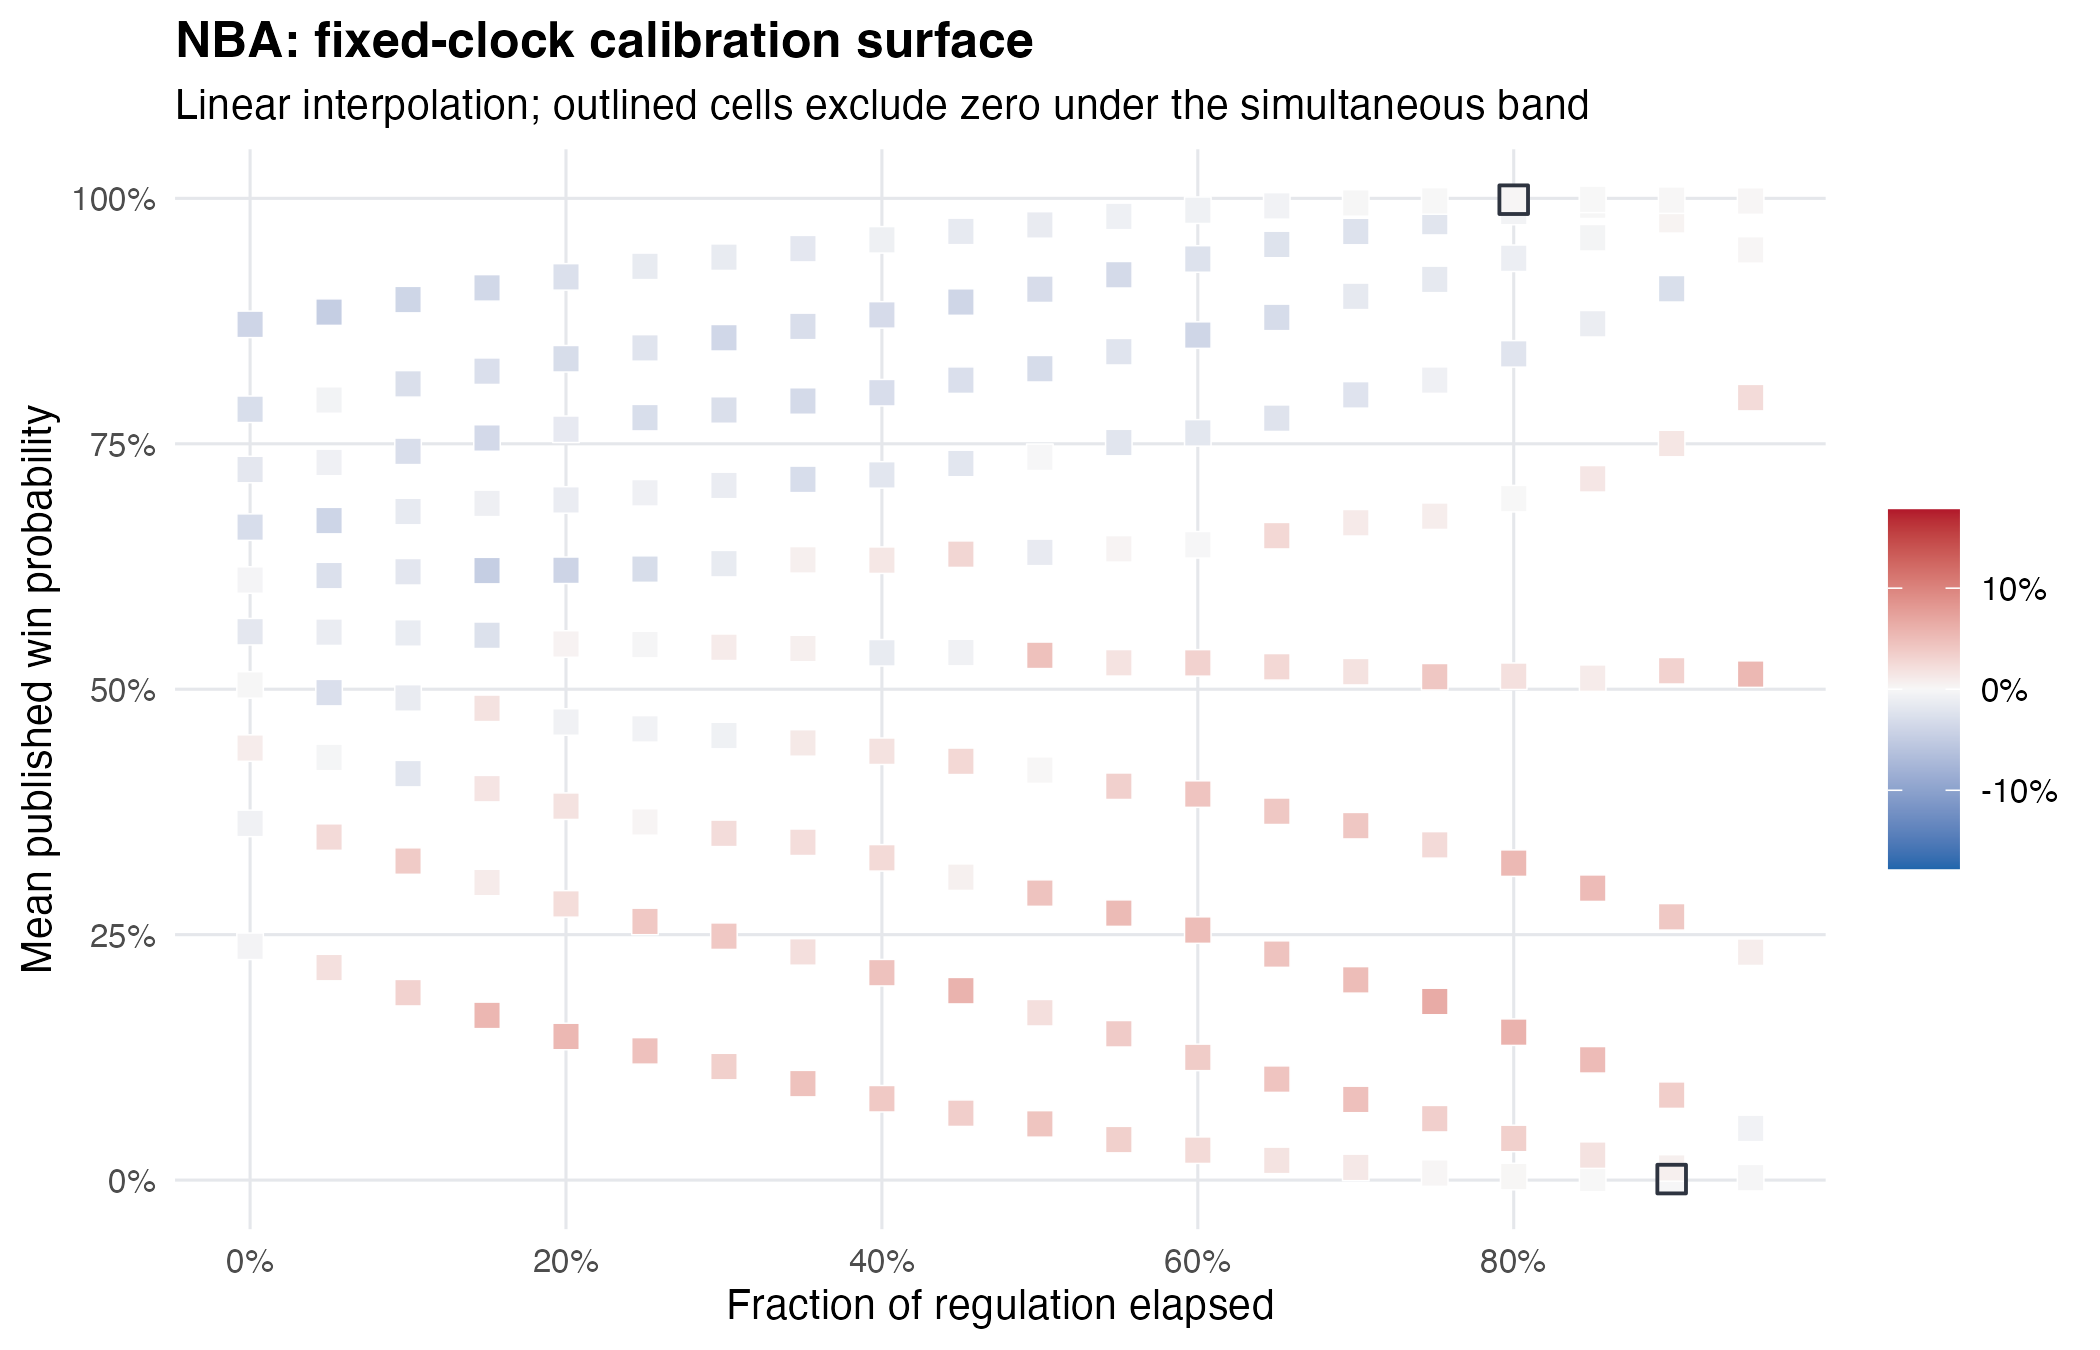
\includegraphics[width=\linewidth]{figures/nba/fixed_clock_surface_linear.png}
  \\[-0.2em]{\small (b) NBA, linear interpolation}
\end{minipage}\\[0.8em]
\begin{minipage}[t]{0.49\linewidth}
  \centering
  
\includegraphics[width=\linewidth]{figures/nfl/fixed_clock_surface_locf.png}
  \\[-0.2em]{\small (c) NFL, LOCF}
\end{minipage}\hfill
\begin{minipage}[t]{0.49\linewidth}
  \centering
  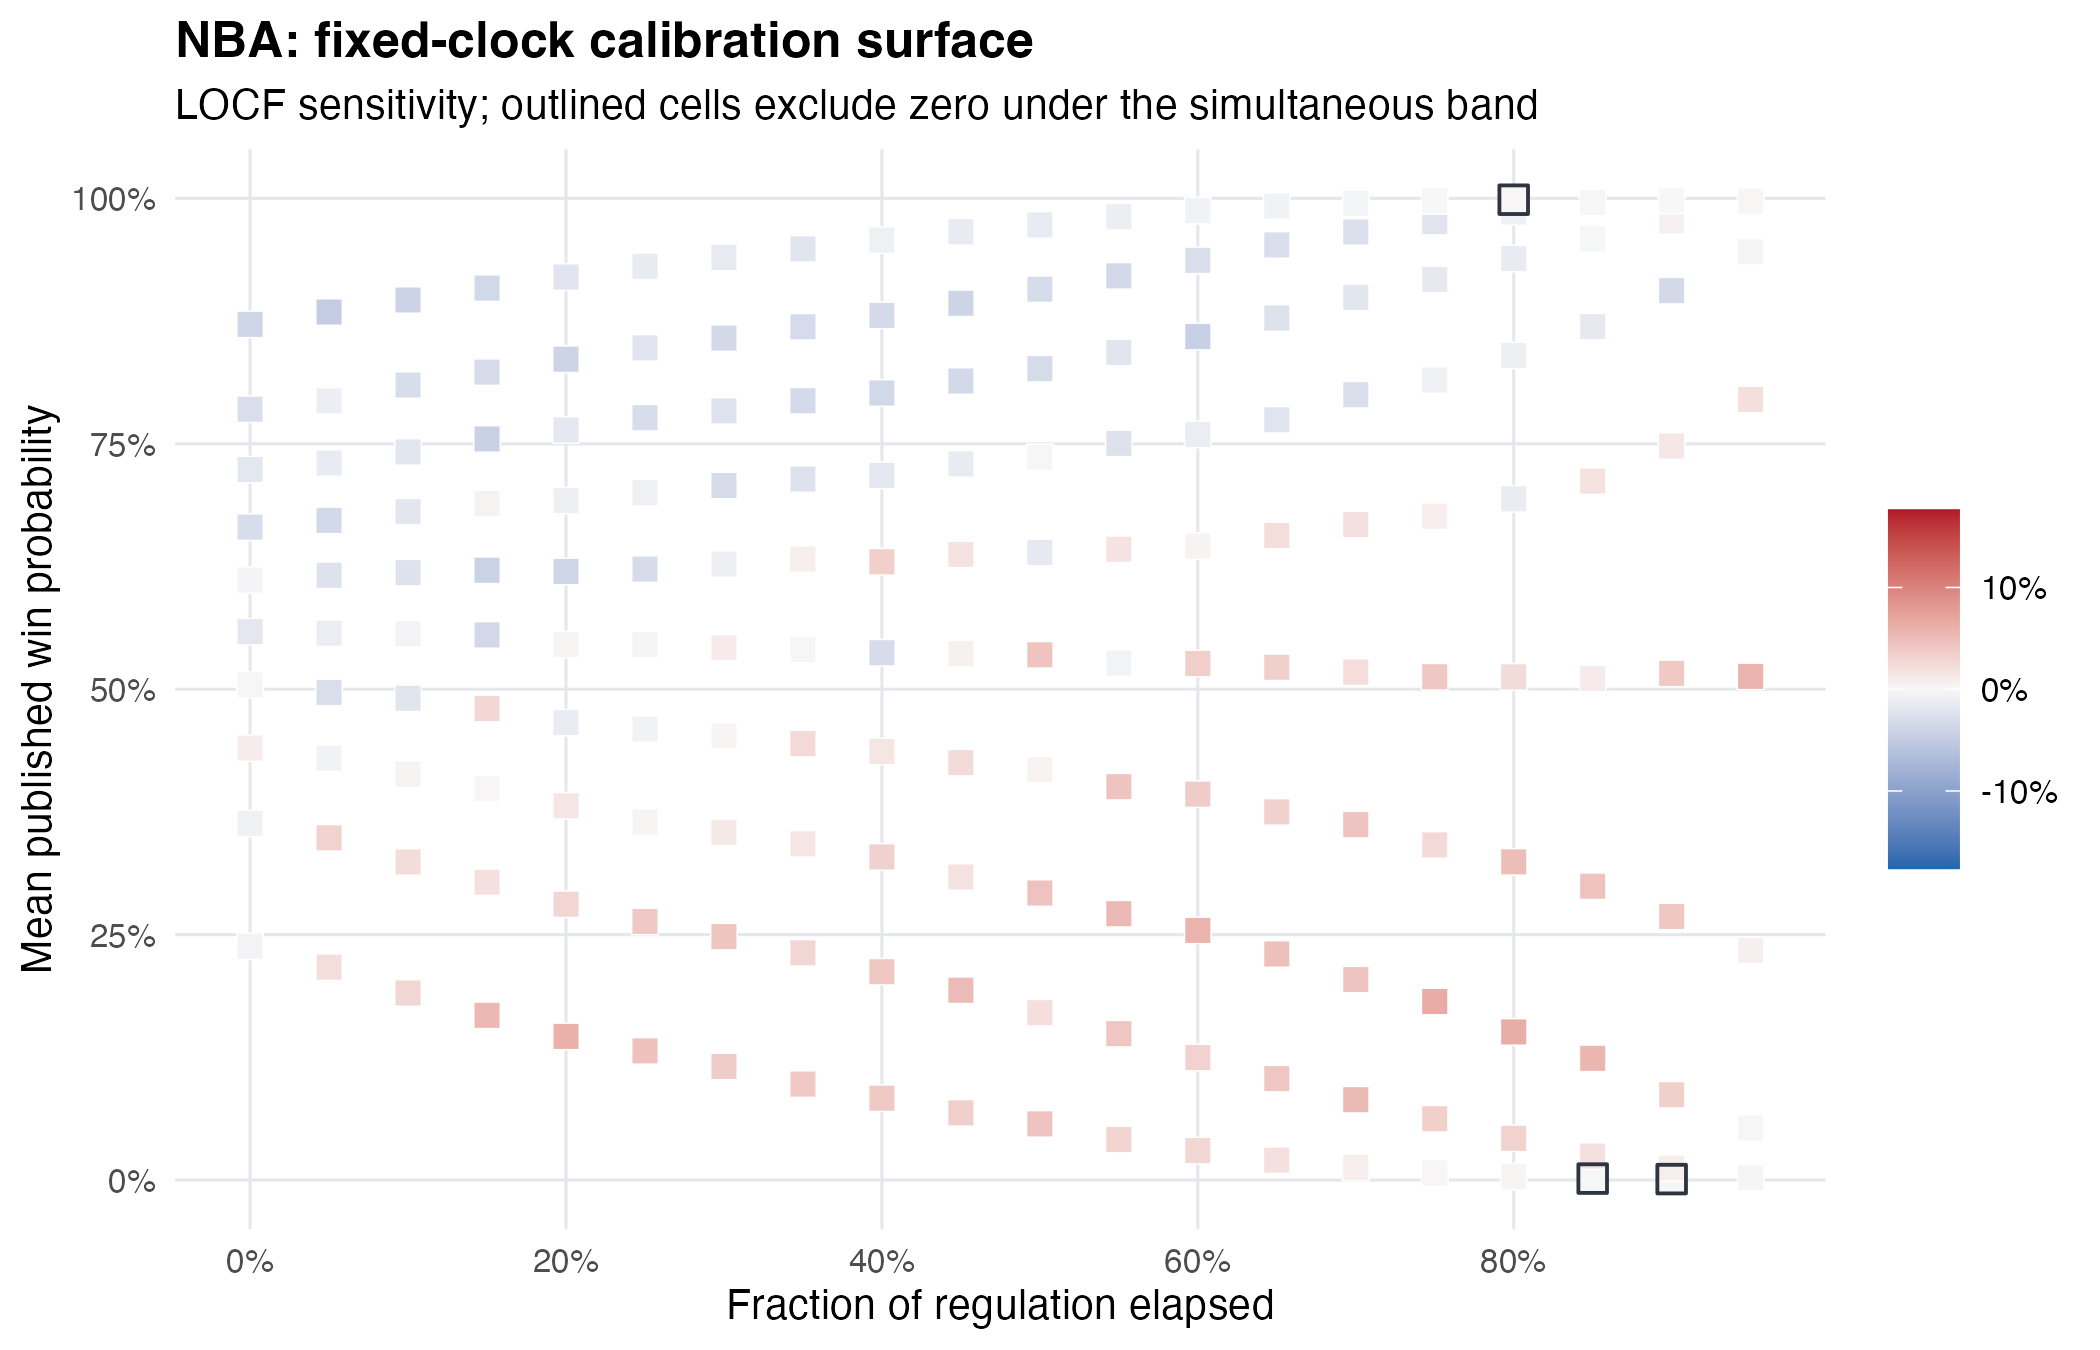
\includegraphics[width=\linewidth]{figures/nba/fixed_clock_surface_locf.png}
  \\[-0.2em]{\small (d) NBA, LOCF}
\end{minipage}
\caption{Fixed-clock calibration surfaces. Color is observed win rate minus mean published probability; outlined cells exclude zero under the simultaneous dyadic band. The bin locations adapt to the forecast distribution at each time.}
\label{fig:supp-fixed-clock}
\end{figure}

The fixed-clock surfaces evaluate reliability at prespecified times; the collapse benchmark evaluates the selected losing path.

\section{Full Collapse Results and Robustness} \label{sec:supp-results}

\subsection{Full tail and first-crossing results}

Table~\ref{tab:supp-tail} reports upper-tail rates at $0.90$, $0.95$, and $0.99$.
The NBA excess is positive at $0.90$ and $0.95$; its $0.99$ interval includes zero.

\begin{table}[!tbp]
\centering
\small
\caption{Upper-tail rates and excess over the continuous benchmark. Intervals are two-sided percentile dyadic-bootstrap intervals for the excess.}
\label{tab:supp-tail}
\begin{tabular}{lcccc}
\hline
League & Threshold & Tail rate & Benchmark rate & Excess (95\% CI) \\
\hline
NFL & 0.90 & \NFLTailNinetyRate & 10.0\% & \NFLTailNinetyExcess{} [\NFLTailNinetyCILower, \NFLTailNinetyCIUpper] \\
NFL & 0.95 & \NFLTailNinetyFiveRate & 5.0\% & \NFLTailNinetyFiveExcess{} [\NFLTailNinetyFiveCILower, \NFLTailNinetyFiveCIUpper] \\
NFL & 0.99 & \NFLTailNinetyNineRate & 1.0\% & \NFLTailNinetyNineExcess{} [\NFLTailNinetyNineCILower, \NFLTailNinetyNineCIUpper] \\
NBA & 0.90 & \NBATailNinetyRate & 10.0\% & \NBATailNinetyExcess{} [\NBATailNinetyCILower, \NBATailNinetyCIUpper] \\
NBA & 0.95 & \NBATailNinetyFiveRate & 5.0\% & \NBATailNinetyFiveExcess{} [\NBATailNinetyFiveCILower, \NBATailNinetyFiveCIUpper] \\
NBA & 0.99 & \NBATailNinetyNineRate & 1.0\% & \NBATailNinetyNineExcess{} [\NBATailNinetyNineCILower, \NBATailNinetyNineCIUpper] \\
\hline
\end{tabular}
\end{table}

For a team-side path, let $\tau_q$ be the first published update at or above $q$ with positive game time remaining.
If no preterminal crossing occurs, set $\tau_q=N$ and retain the indicator of crossing.
Because $\tau_q$ is bounded and $\{\tau_q<N\}\in\mathcal F_{\tau_q}$, sequential calibration implies
\[
\E\{(p_{\tau_q}-Y)\mathbf 1(\tau_q<N)\}=0.
\]
Optional stopping therefore centers the first-crossing residual at zero under sequential calibration.
Table~\ref{tab:supp-crossing} reports $\overline{1-Y}$, $\overline{1-p_{\tau_q}}$, and their difference $\bar R=\overline{p_{\tau_q}-Y}$.
The estimand is an average over crossing episodes; when two episodes come from the same game, they receive the same dyadic game weight.
The crossing estimand uses a published probability $p\ge q$; the tail estimand in Table~\ref{tab:supp-tail} uses the game-level benchmark score $U\ge q$.

\begin{table}[!tbp]
\centering
\small
\setlength{\tabcolsep}{4pt}
\caption{Preterminal first crossings. The interval is for the mean residual $\bar R$.}
\label{tab:supp-crossing}
\begin{tabular}{lcrrrrr}
\hline
League & $q$ & Episodes & Games & Observed loss & Implied loss & $\bar R$ (95\% CI) \\
\hline
NFL & 0.90 & \NFLCrossingNinetyEpisodes & \NFLCrossingNinetyGames & \NFLCrossingNinetyLoss & \NFLCrossingNinetyImplied & \NFLCrossingNinetyResidual{} [\NFLCrossingNinetyCILower, \NFLCrossingNinetyCIUpper] \\
NFL & 0.95 & \NFLCrossingNinetyFiveEpisodes & \NFLCrossingNinetyFiveGames & \NFLCrossingNinetyFiveLoss & \NFLCrossingNinetyFiveImplied & \NFLCrossingNinetyFiveResidual{} [\NFLCrossingNinetyFiveCILower, \NFLCrossingNinetyFiveCIUpper] \\
NFL & 0.99 & \NFLCrossingNinetyNineEpisodes & \NFLCrossingNinetyNineGames & \NFLCrossingNinetyNineLoss & \NFLCrossingNinetyNineImplied & \NFLCrossingNinetyNineResidual{} [\NFLCrossingNinetyNineCILower, \NFLCrossingNinetyNineCIUpper] \\
NBA & 0.90 & \NBACrossingNinetyEpisodes & \NBACrossingNinetyGames & \NBACrossingNinetyLoss & \NBACrossingNinetyImplied & \NBACrossingNinetyResidual{} [\NBACrossingNinetyCILower, \NBACrossingNinetyCIUpper] \\
NBA & 0.95 & \NBACrossingNinetyFiveEpisodes & \NBACrossingNinetyFiveGames & \NBACrossingNinetyFiveLoss & \NBACrossingNinetyFiveImplied & \NBACrossingNinetyFiveResidual{} [\NBACrossingNinetyFiveCILower, \NBACrossingNinetyFiveCIUpper] \\
NBA & 0.99 & \NBACrossingNinetyNineEpisodes & \NBACrossingNinetyNineGames & \NBACrossingNinetyNineLoss & \NBACrossingNinetyNineImplied & \NBACrossingNinetyNineResidual{} [\NBACrossingNinetyNineCILower, \NBACrossingNinetyNineCIUpper] \\
\hline
\end{tabular}
\end{table}

\subsection{Feed and specification sensitivity}

Table~\ref{tab:supp-specification} reports sensitivity to feed corrections, rounding, dependence structure, threshold convention, and time sampling.
The crossing rows report the $0.95$ residual, while the fixed-clock rows report descriptive root-mean-square calibration gaps over time--probability cells.
For reported probabilities rounded to three decimals, lower and upper PIT vectors are obtained by allowing each probability to range within $\pm0.0005$ and using monotonicity of the benchmark transform.
The dyad-plus-calendar row multiplies the team multiplicity by a circular two-week block multiplicity within each season, retaining team dependence while allowing common model-period shocks.
The franchise-linked row maps relocations to a common franchise and applies one team multiplicity across all seasons, allowing persistent team effects.

\begin{table}[!tbp]
\centering
\small
\setlength{\tabcolsep}{4pt}
\caption{Feed and specification sensitivity. Brackets denote 95\% intervals where shown.}
\label{tab:supp-specification}
\begin{tabular}{lll}
\hline
Specification & NFL & NBA \\
\hline
Global, corrected: $D$ ($p$) & \NFLGlobalD{} (\NFLGlobalDyadicP) & \NBAGlobalD{} (\NBAGlobalDyadicP) \\
Global, raw: $D$ ($p$) & \NFLRawGlobalD{} (\NFLRawGlobalP) & \NBARawGlobalD{} (\NBARawGlobalP) \\
Exclude patched games: $D$ ($p$) & \NFLExcludePatchedGlobalD{} (\NFLExcludePatchedGlobalP) & \NBAExcludePatchedGlobalD{} (\NBAExcludePatchedGlobalP) \\
Rounding bound for $D$ & [\NFLRoundingLowerGlobalD, \NFLRoundingUpperGlobalD] & [\NBARoundingLowerGlobalD, \NBARoundingUpperGlobalD] \\
Rounding bound for $\widehat\P(U\ge.95)$ & [\NFLRoundingLowerTailNinetyFiveRate, \NFLRoundingUpperTailNinetyFiveRate] & [\NBARoundingLowerTailNinetyFiveRate, \NBARoundingUpperTailNinetyFiveRate] \\
Dyad plus calendar: $D$ ($p$) & \NFLDyadicCalendarGlobalD{} (\NFLDyadicCalendarGlobalP) & \NBADyadicCalendarGlobalD{} (\NBADyadicCalendarGlobalP) \\
Franchise linked: $D$ ($p$) & \NFLFranchiseLinkedGlobalD{} (\NFLFranchiseLinkedGlobalP) & \NBAFranchiseLinkedGlobalD{} (\NBAFranchiseLinkedGlobalP) \\
Crossing, preterminal $p\ge.95$ & \NFLCrossingNinetyFiveResidual{} [\NFLCrossingNinetyFiveCILower, \NFLCrossingNinetyFiveCIUpper] & \NBACrossingNinetyFiveResidual{} [\NBACrossingNinetyFiveCILower, \NBACrossingNinetyFiveCIUpper] \\
Crossing, preterminal $p>.95$ & \NFLCrossingNinetyFiveStrictResidual{} [\NFLCrossingNinetyFiveStrictCILower, \NFLCrossingNinetyFiveStrictCIUpper] & \NBACrossingNinetyFiveStrictResidual{} [\NBACrossingNinetyFiveStrictCILower, \NBACrossingNinetyFiveStrictCIUpper] \\
Crossing, terminal-inclusive & \NFLCrossingNinetyFiveAllResidual{} [\NFLCrossingNinetyFiveAllCILower, \NFLCrossingNinetyFiveAllCIUpper] & \NBACrossingNinetyFiveAllResidual{} [\NBACrossingNinetyFiveAllCILower, \NBACrossingNinetyFiveAllCIUpper] \\
Fixed clock, linear RMS & \NFLFixedClockLinearRMS & \NBAFixedClockLinearRMS \\
Fixed clock, LOCF RMS & \NFLFixedClockLOCFRMS & \NBAFixedClockLOCFRMS \\
\hline
\end{tabular}
\end{table}

At $0.95$, strict versus weak tail counting differs only through the observed atom: the weak and strict NBA rates are \NBATailNinetyFiveRate{} and \NBATailNinetyFiveStrictRate{}, with \NBATailNinetyFiveAtomRate{} exactly at the boundary; the corresponding NFL values are \NFLTailNinetyFiveRate{}, \NFLTailNinetyFiveStrictRate{}, and \NFLTailNinetyFiveAtomRate{}.
The path audit identified \NBAPatchedGames{} NBA and \NFLPatchedGames{} NFL games containing loser-side exact-one feed values.
The raw, corrected, and exclusion rows in Table~\ref{tab:supp-specification} use identical team draws.

\subsection{Season persistence}

The acquisition ledger in Table~\ref{tab:supp-coverage} gives explicit missing-feed accounting for both leagues.
NFL coverage is complete; minimum NBA season coverage is \NBAMinimumFeedCoverage{}.

Table~\ref{tab:supp-loso} gives descriptive stability summaries after omitting one season at a time.
Across omissions, the NBA global statistic ranges from \NBALOSODMin{} to \NBALOSODMax{}, while the NFL statistic ranges from \NFLLOSODMin{} to \NFLLOSODMax{}.

\begin{table}[!tbp]
\centering
\small
\caption{Leave-one-season-out global statistic and $0.95$ tail excess.}
\label{tab:supp-loso}
\begin{minipage}[t]{0.47\linewidth}
\centering
\textbf{NFL}\\[0.3em]
\begin{tabular}{lrrr}
\hline
Omitted & Games & $D$ & Excess \\
\hline
\NFLLeaveSeasonRows
\hline
\end{tabular}
\end{minipage}\hfill
\begin{minipage}[t]{0.47\linewidth}
\centering
\textbf{NBA}\\[0.3em]
\begin{tabular}{lrrr}
\hline
Omitted & Games & $D$ & Excess \\
\hline
\NBALeaveSeasonRows
\hline
\end{tabular}
\end{minipage}
\end{table}

\FloatBarrier
Across specifications, the NBA departure remains a recurrent upper-tail feature.
The tail excess is positive at $0.90$ and $0.95$, first-crossing residuals are positive at all three thresholds, and the global test rejects for the raw paths, corrected paths, patched-game exclusion, calendar blocks, and franchise linkage.
Across the leave-one-season-out samples, $D_n^{\mathrm{upper}}$ ranges from \NBALOSODMin{} to \NBALOSODMax{} and the $0.95$ tail excess ranges from \NBALOSOTailMin{} to \NBALOSOTailMax{}.
The game-level $0.99$ tail interval includes zero, marking the limit of the upper-tail evidence.
Across specifications, the NFL retains the global conclusion of no detected departure; its positive $0.99$ first-crossing residual is a localized result.

\section{Finite-Schedule Null Simulation} \label{sec:supp-validation}

Finite-sample Type I error is evaluated while retaining the teams and matchups in each observed season schedule.
For game $g$ between teams $a_g$ and $b_g$, generate
\[
Z_g=\sqrt{\rho}\,(A_{s,a_g}+A_{s,b_g})/\sqrt{2}
    +\sqrt{1-\rho}\,E_g,
\qquad U_g=\Phi(Z_g),
\]
where team effects and game shocks are independent standard normals and team effects are redrawn by season.
Marginally, $Z_g$ is standard normal and $U_g$ is uniform, placing every simulation on the boundary of the continuous calibration null.
Games sharing a team are correlated through the team effect, with $\rho$ controlling the strength of that dependence.
For each $\rho\in\{0,0.25,0.5\}$, the global test is applied to \ValidationOuterSamples{} Monte Carlo samples using \ValidationInnerReplicates{} inner pigeonhole draws.
The proportion rejected estimates finite-schedule Type I error at nominal level 5\%.
When $\rho=0$, the pigeonhole procedure is expected to be conservative because the dyadic projection is degenerate; this is the regime in which multiway bootstrap behavior requires particular care \citep{Menzel2021}.
Table~\ref{tab:supp-validation} reports the resulting rejection rates.

\begin{table}[!tbp]
\centering
\caption{Empirical 5\% rejection rates in the finite-schedule null simulation (\ValidationOuterSamples{} Monte Carlo samples; \ValidationInnerReplicates{} inner draws).}
\label{tab:supp-validation}
\begin{tabular}{lcc}
\hline
League & $\rho$ & Dyadic rejection rate \\
\hline
NFL & 0 & \ValidationNFLRhoZeroDyadic \\
NFL & 0.25 & \ValidationNFLRhoTwentyFiveDyadic \\
NFL & 0.5 & \ValidationNFLRhoFiftyDyadic \\
NBA & 0 & \ValidationNBARhoZeroDyadic \\
NBA & 0.25 & \ValidationNBARhoTwentyFiveDyadic \\
NBA & 0.5 & \ValidationNBARhoFiftyDyadic \\
\hline
\end{tabular}
\end{table}
The test is conservative under these schedule-specific nulls.
Rejection rates rise with the shared-team component, from \ValidationNFLRhoZeroDyadic{} to \ValidationNFLRhoFiftyDyadic{} on the NFL schedule and from \ValidationNBARhoZeroDyadic{} to \ValidationNBARhoFiftyDyadic{} on the NBA schedule, remaining at or below the nominal 5\% level.
The simulation targets finite-schedule size under shared-team dependence; calendar and cross-season dependence are examined through the sensitivities in Section~\ref{sec:supp-results}.

\bibliographystyle{imsart-nameyear}
\bibliography{references}
\end{document}
